\documentclass[a4paper,11pt]{beamer}
\usepackage[spanish,activeacute]{babel}
\usepackage[utf8]{inputenc}
\usepackage{amsmath,amsthm}
\usepackage{amsfonts,amssymb}
\usepackage{beamerthemesplit}
\usetheme{Madrid} % tema a escoger
\usecolortheme{default} % colores: probar crane, dove, beetle y dolphin, por ejemplo
\usefonttheme{professionalfonts} % fuente para ecuaciones
\usepackage{graphicx}
\usepackage{enumerate,array}

\usepackage{tikz}
\usetikzlibrary{shapes,arrows}
\usetikzlibrary{babel}


\newtheorem{proposition}{Proposición}[section]

% \setbeamertemplate{caption}[numbered]{} % esto es para que numere las tablas y las figuras

 \setbeamercovered{transparent=5}

\author[ Mario Muñoz Mesa]{Mario Muñoz Mesa}
\title[Grey Wolf Optimizer]{Práctica Alternativa: Grey Wolf Optimizer}
\date{}

%\institute{Metaheurísticas.}

\AtBeginSection{
	\frame{\frametitle{Índice de contenidos} % es para que al inicio de cada sección haya un índice (y su nombre)
	\tableofcontents[currentsection]}
}

\begin{document}
\maketitle

\frame{
 \tableofcontents
}

\section{Grey Wolf Optimizer (GWO).}

\begin{frame}{Grey Wolf Optimizer (GWO).}
    \begin{itemize}
        \item Técnica tipo Swarm Intelligence.
        \item GWO está inspirado en la jerarquía social y de comportamiento de caza de manadas de lobo gris.
    \end{itemize}
\end{frame}

\section{Inspiración.}

\begin{frame}{Inspiración.}
    Grandes depredadores que viven en manadas de 5 a 12 en promedio. Conviven en una jerarquía social dominante:
    \begin{figure}[H]
		\centering
		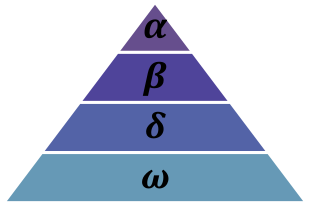
\includegraphics[width=0.35\textwidth]{images/jerarq.png}
		\caption{Jerarquía, más dominante arriba.}
	\end{figure}
	Fases de caza:
	\begin{itemize}
		\item Rastrear, seguir y acercarse a la presa.
		\item Perseguir, rodear y hostigar a la presa hasta que deje de moverse.
		\item Atacar a la presa.
	\end{itemize}

    ~\\

\end{frame}



\section{Jerarquía social - Modelo matemático.}

\begin{frame}{Jerarquía social - Modelo matemático.}
    Para modelar matemáticamente: primera solución alpha, segunda beta, tercera delta. El resto de soluciones omega. La caza estará guiada por $\alpha$, $\beta$ y $\delta$
    
\end{frame}

\subsection{Rodear a la presa - Modelo Matemático.}

\begin{frame}{Rodear a la presa - Modelo Matemático.}
    Ecuaciones para modelar el rodeo de los lobos grises a su presa durante la caza:
    $$\vec{D} = |\vec{C} \cdot \vec{X}_p(t)-\vec{X}(t)|$$
	$$\vec{X}(t+1)=\vec{X}_p(t)-\vec{A}\cdot \vec{D}$$
	donde $t$ es la iteración actual, $\vec{A}$ y $\vec{C}$ vectores de coeficientes reales, $\vec{X}_p$  es el vector de posición de la presa, y $\vec{X}$ denota el vector de posición de un lobo gris.
	
	$\vec{A}$ y $\vec{C}$ se calculan como:
	$$\vec{A}=2\vec{a}\cdot \vec{r}_1 -\vec{a}$$
	$$\vec{C}=2\cdot \vec{r}_2$$
	donde $\vec{a}$ decrementa linealmente de 2 a 0 en el transcurso de iteraciones y $\vec{r}_1$, $\vec{r}_2$ son vectores aleatorios con valores en $[0,1]$ (unidimensionales). 

\end{frame}

\begin{frame}{Rodear a la presa - Modelo Matemático.}
	Con las ecuaciones propuestas, un lobo gris en posición $(X,Y)$ puede actualizar su posición en base a la posición de la presa $(X^*, Y^*)$
    \begin{figure}[H]
		\centering
		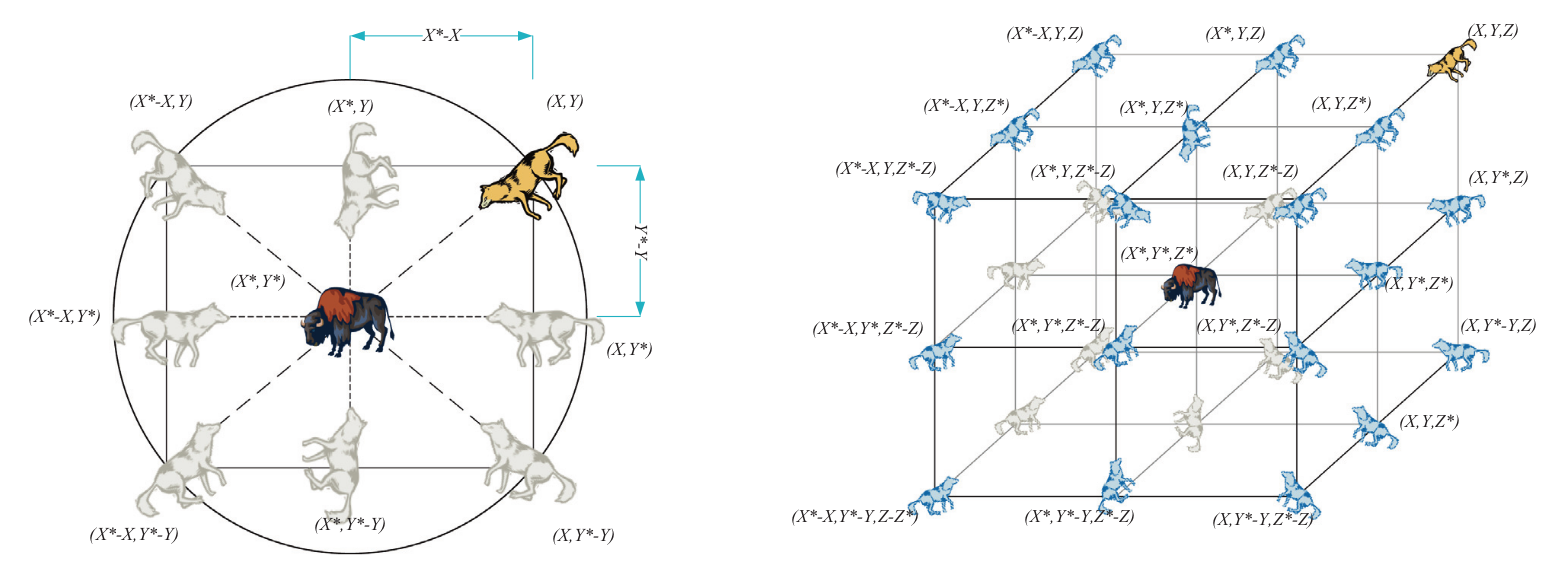
\includegraphics[width=1\textwidth]{images/2d_3d.png}
	\end{figure} 
	$\vec{r}_1$ y $\vec{r}_2$ permiten cualquier posición intermedia a las ilustradas. Así un lobo gris podría moverse alrededor de la mejor posición hasta el momento a cualquier posición en el espacio de búsqueda usando las ecuaciones anteriores.

\end{frame}


\subsection{Cazar - Modelo matemático.}

\begin{frame}{Cazar - Modelo Matemático.}
	Para modelar la caza, como no se sabe la localización de la presa, se supone que el alpha, beta y delta tienen mejor conocimiento de la localización de la presa (esas posiciones se guardarán). Las fórmulas propuestas:
	$$\vec{D}_{\alpha} = |\vec{C}_1\cdot \vec{X}_{\alpha} - \vec{X}|, \quad \vec{D}_{\beta} = | \vec{C}_2\cdot \vec{X}_{\beta}-\vec{X}|, \quad \vec{D}_{\delta} = |\vec{C}_3\cdot \vec{X}_{\delta} - \vec{X}|$$
	$$\vec{X}_1 = \vec{X}_{\alpha} - \vec{A}_1 \cdot (\vec{D}_{\alpha}), \quad \vec{X}_2 = \vec{X}_{\beta} - \vec{A}_2 \cdot (\vec{D}_{\beta}), \quad \vec{X}_3=\vec{X}_{\delta} - \vec{A}_3 \cdot (\vec{D}_{\delta})$$
	$$\vec{X} (t+1) = \frac{\vec{X}_1 + \vec{X}_2 + \vec{X}_3}{3} \quad \quad \ \ (3.7)$$

\end{frame}




\begin{frame}{Cazar - Modelo matemático}
     \begin{figure}[H]
		\centering
		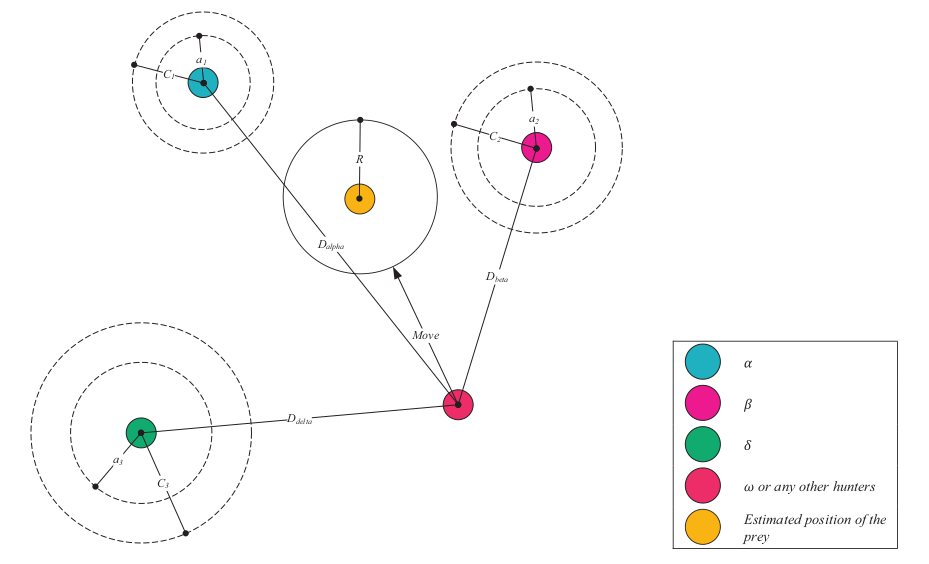
\includegraphics[width=0.9\textwidth]{images/omega_movement.png}
		\caption{Actualización de posición.}
	\end{figure}
\end{frame}

\subsection{Explotación y exploración.}

\begin{frame}{Explotación.}
	\begin{itemize}
		\item Atacar la presa (explotación). Los lobos grises finalizan la caza atacando a la presa cuando deja de moverse. $\vec{A}$ decrementa por $a$, $\vec{A}$ toma valor aleatorio en $[-2a, 2a]$, donde $a$ decrementa de 2 a 0 durante las iteraciones. Cuando $|\vec{A}|<1$ el lobo ataca a la presa, la siguiente posición del agente estará entre la suya y la de la presa.
	\end{itemize}

\end{frame}

\begin{frame}{Exploración.}
	\begin{itemize}
		\item Buscar a la presa (exploración). 	Los lobos grises mayormente buscan en base a la posición de alpha, beta y delta. Divergen entre sí para buscar la presa y convergen para atacarla. Cuando $|\vec{A}|>1$ el agente buscador diverge de la presa. Esto enfatiza la exploración. \\
	
		\item Otra componente que favorece la exploración es $\vec{C}$ que toma valores en $[0,2]$. Esta componente provee pesos aleatorios para acentuar ($|\vec{C}|>1$) o minorar ($|\vec{C}|<1$) el efecto de la presa. Esto ayuda a que GWO tenga un comportamiento más aleatorio, favoreciendo la exploración y evitando quedar atrapado en óptimos locales.
	\end{itemize}

\end{frame}


\section{Pseudocódigo.}
\begin{frame}{Pseudocódigo} 
	 \begin{itemize}
	 	\item El proceso de búsqueda comienza creando una población de lobos grises (soluciones candidatas). 
	 	\item Conforme se itera, los lobos alpha, beta y delta estiman la probable posición de la presa. 
	 	\item Cada solución candidata actualiza su posición a la presa. 
	 	\item El parámetro $a$ decrementa de 2 a 0 para enfatizar la exploración y explotación respectivamente. 
	 	\item Las soluciones candidatas tienden a diverger de la presa cuando $|\vec{A}|>1$ y converger cuando $|\vec{A}|<1$. 
	 	\item Finalmente el algoritmo termina con una condición de parada como puede ser un máximo de iteraciones.
	\end{itemize}
	

\end{frame}

\begin{frame}{Pseudocódigo}
    \begin{figure}[H]
		\centering
		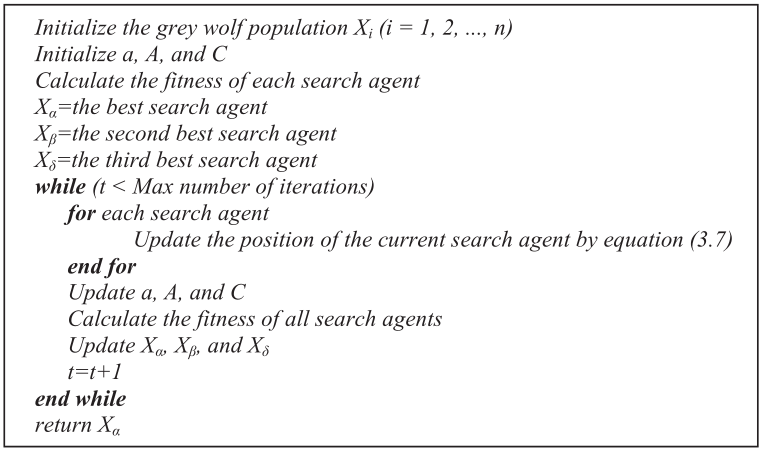
\includegraphics[width=0.8\textwidth]{images/gwo_pseudocode.png}
		\caption{Pseudocódigo.}
	\end{figure}.    
\end{frame}



\end{document}
